Simulated annealing is a probabilistic technique for approximating the global optimum of a given function, in other word,it attempts to find the global optimum in presence of multiple local optima.\\
The aim of this exercise is finding a route S (a permutation of $1, . . . , n$) with minimal total cost $\Sigma^{i=1}_{n_1}A(S_{i},S_{i+1})$ in Travelling salesman problem (TSP) with Given n stations, and an n-by-n matrix A giving the cost of going
from station i to j, which starts and ends at station 1, $S1 = 1$.\\

Three parameters "tempMax", "coefDecay" and "coefStretch" are added in the function to calculate the decreasing temperature. The main purpose is to lower the annealing speed, which allows more "jumping" from the local optimal in the early stage.

\begin{lstlisting}
function [temp] = calTemp(k, tempMax, coefDecay, coefStretch)
    temp = tempMax / (1 + coefStretch * k)^coefDecay;
end
\end{lstlisting}

\begin{center}
    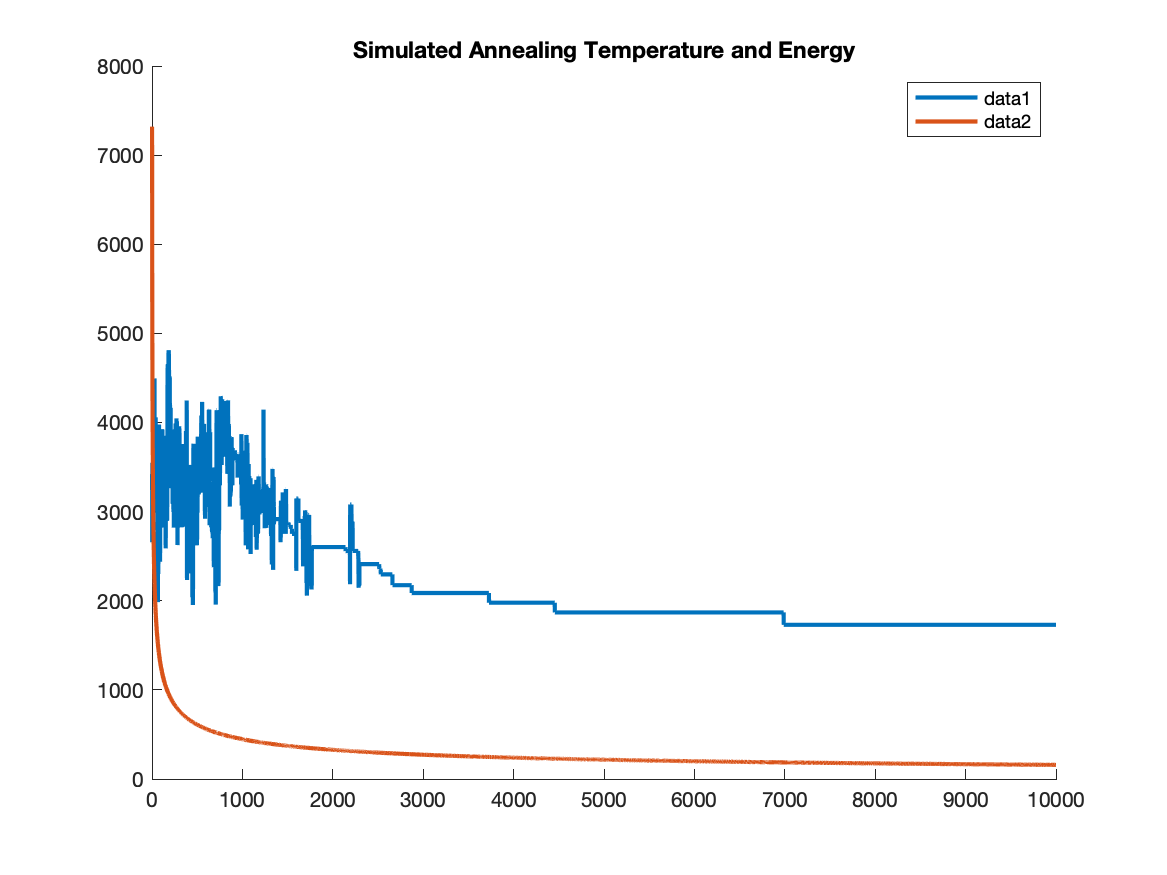
\includegraphics[scale=0.5]{Figures/figure7_3.png}\\
    \figuretitle{Figure 18: simulated Annealing temperature and energy.}
\end{center}\\

Once there are enough "jump" for searching, we extend the simulation times to try to get better result.

\begin{center}
    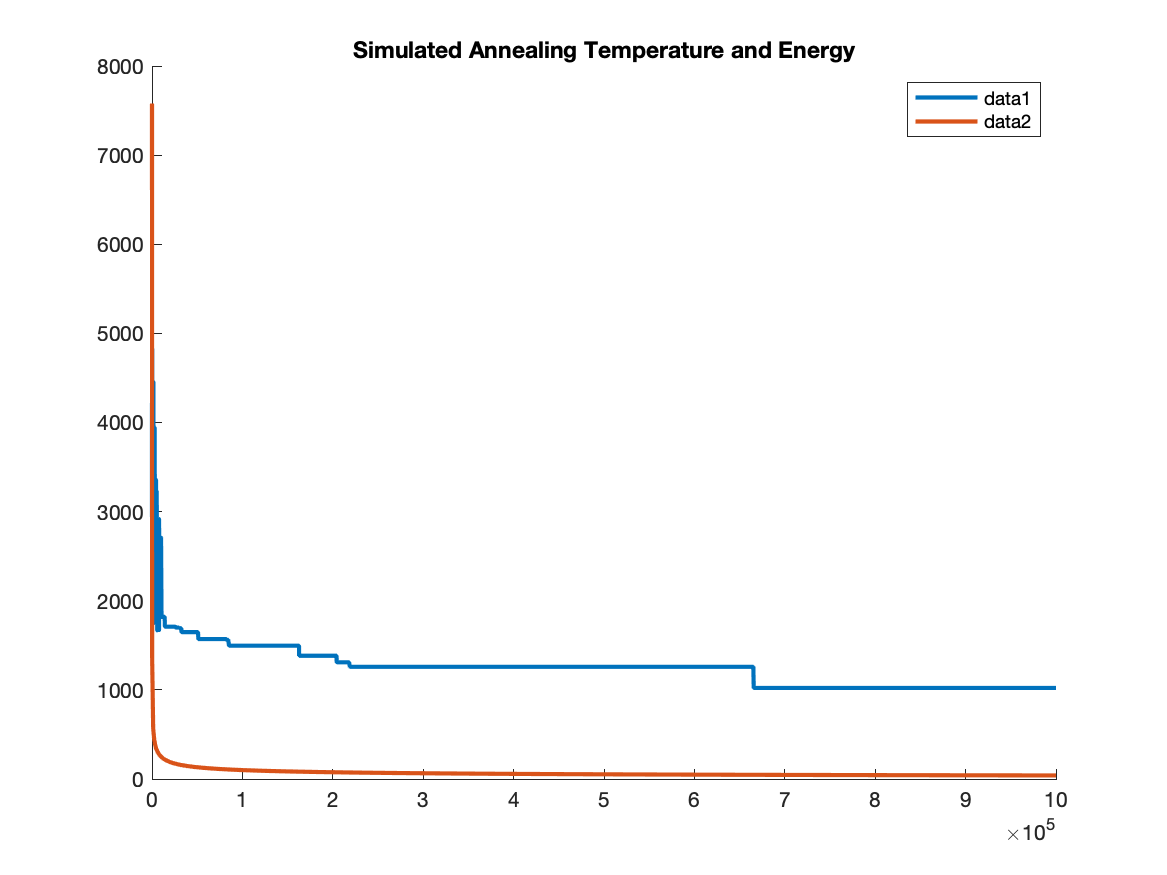
\includegraphics[scale=0.5]{Figures/figure7_1.png}\\
    \figuretitle{Figure 19: simulated Annealing temperature and energy.}
\end{center}\\

The final result from experiment is shown in the following table:

\begin{center}
    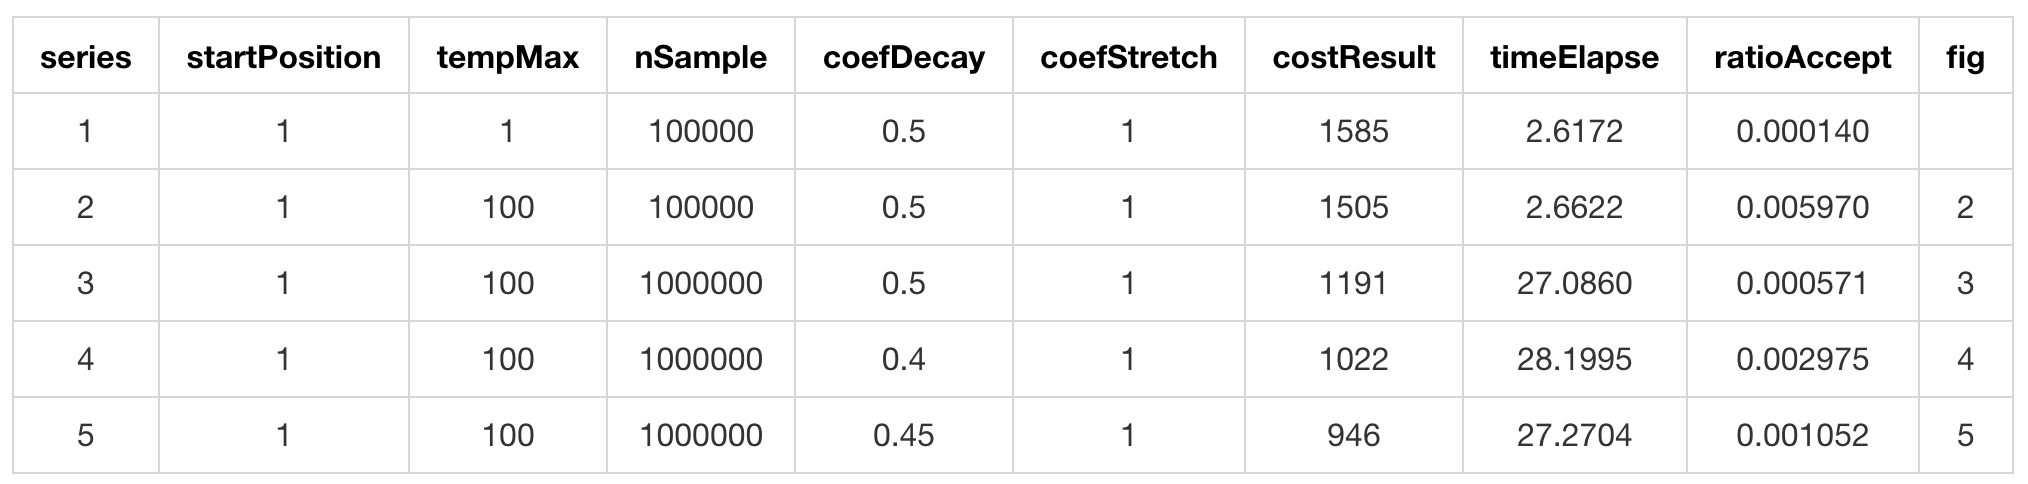
\includegraphics[scale=0.5]{Figures/figure7_2.png}\\
    \figuretitle{Table 8: Optimization Result.}
\end{center}\\